\documentclass[a4paper, 12pt]{article}
\usepackage{geometry}
\geometry{margin=2cm}
\usepackage[indonesian]{babel}
\usepackage{setspace}
\onehalfspacing{}
\usepackage{hyperref}
\usepackage{float}
\hypersetup{
    colorlinks,
    citecolor=black,
    filecolor=black,
    linkcolor=blue,
    urlcolor=blue
}

\usepackage{graphicx}
\graphicspath{./images/}
\title{\textbf{Tugas UAS}\linebreak
\textbf{Konfigurasi Access point Achmad}\linebreak}
\date{}

\usepackage{subfiles}
% \usepackage{indentfirst}
\setlength{\parindent}{20pt}
\begin{document}
\subfile{./subfiles/cover.tex}

% \tableofcontents
% \thispagestyle{empty}
% \pagebreak
\clearpage
\section{Tugas}
Pada sebuah kantor seorang manajer bernama Achmad menginginkan ruanganny memiliki jaringan hotspot tersendiri, berbeda dengan bawahannya. Achmad menginginkan hanya ada 6 clients saja yang dapat terkoneksi dengan access point tersebut. meskipun sudah dibatasi dengan penggunaan \textit{mac filtering} pada 6 clients, Achmad masih tidak puas dan menginginkan hotspotnya memiliki \textit{password security}\dots Achmad mengetahui bahwa ada bawahannya yang mengerti tentang \textit{hacking} pada jaringan \textit{wireless}\dots Pada suatu waktu Achmad menyadari bahwa hotspotnya memiliki pengunjung gelap. Achmad mengetahui \textit{mac address} pengunjung gelap tersebut dan menginginkan pengunjung gelap tersebut tidak dapat terkoneksi ke hotspot milikinya. Koneksi internet hotspot tersebut didapat dari \textit{access point} di ruang IT. kedua \textit{acces point} (AP IT dan AP ruangan Achmad) harus di konfigurasi terlebih dahulu agar ruangannya memiliki koneksi internet. Berikanlah solusi untuk hal tersebut. diatas
\section{Penyelesaian}
\subsection{Penjabaran}
Berdasarkan informasi diatas maka harus mengkonfigurasi:
\begin{enumerate}
  \item Mengkonfigurasi \textit{Access Point} agar terkoneksi dengan internet\dots
  \item membatasi pengguna maksimal 6 pengguna dengan \textit{Mac filtering}\dots
  \item menambahkan \textit{password security} pada \textit{access point}\dots
  \item mengatasi \textit{hacker} pada jaringan di \textit{acces point} Ruang IT agar tidak terhubung dengan hotspot\dots
\end{enumerate}
\subsection{Mengkonfigurasi \textit{Access Point} agar terhubung dengan internet}
% Untuk menghubungkan jaringan ini dengan internet maka harus ditentukan dahulu Host dari jaringan ini dan Acces point lainnya sebagai \textit{repeater} agar memudahkan proses konfigurasi\dots oleh sebab itu maka Ruangan Achmad menjadi Hostnya dan Ruangan IT menjadi Repeaternyakemudian \textit{access point} Achmad terhubung dengan koneksi fiber dengan provider internet untuk mendapatkan koneksi internet dan menerima \textit{IP Public} untuk menjelajah internet\dots
untuk menghubungkan \textit{Access Point} agar terhubung dengan internet langkah pertama yakni memiliki koneksi internet dari provider yang ada, contohnya indihome yang nantinya akan memberikan akses internet melalui jalur \textit{Fiber Optic} yang nantinya dapat digunakan oleh router untuk mengakses internet\dots
kemudian konfigurasikan \textit{Access Point} yang berada di ruangan IT sebagai Host yang menjadi sarana utama dari Router lain seperti yang berada di ruangan Achmad untuk terhubung ke internet jadi tidak perlu menambah layanan internet ke provider. setelah itu konfigurasikan \textit {Access Point} untuk menerima IP public yang diberikan oleh provider untuk mengakses internet, kemudian konfigurasikan \textit{Access Point} yang berada di ruangan Acmhad sebagai Repeaternya. Untuk mendapatkan \textit{IP Private} untuk saling koneksi pada jaringan lokal maka \textit{Access Point} Host yakni yang ada di Ruang IT menjalankan sistem NAT (Network Address Translation) agar dapat mendapatkan \textit{IP Private} yang dapat membagikan internet kepada perangkat lokal dengan memberikan \textit{IP Private} yang unik pada setiap perangkat.
\begin{figure}[H]
  \begin{center}
    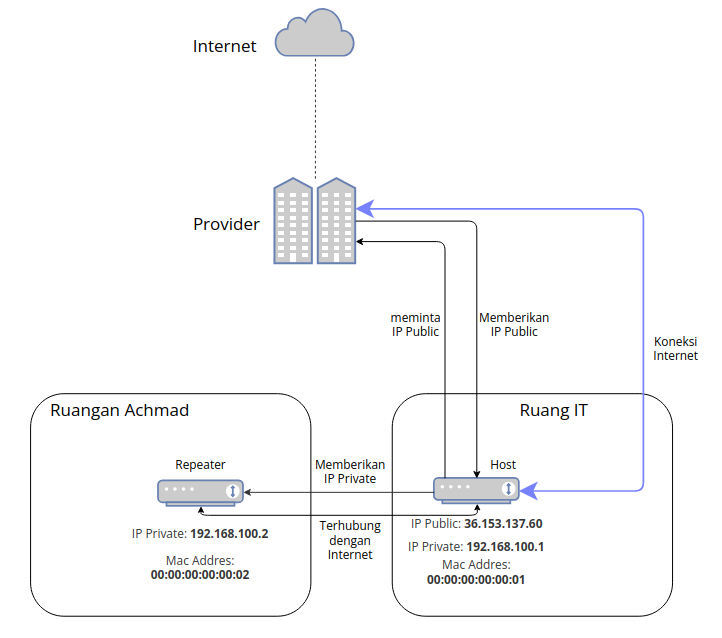
\includegraphics[width=0.95\textwidth]{images/gambar1_2.png}
  \end{center}
  \caption{Gambar Koneksi antara \textit{Access Point} ruang Acmhad dan Ruang IT agar terhubung dengan internet}\label{fig:accespoint}
\end{figure}
berdasarkan gambar \ref{fig:accespoint} dapat terlihat bahwa \textit{access point} ruang Acmhad dan Ruang IT terhubung dengan internet\dots
\subsection{Menambahkan \textit{password security} pada \textit{Access Point}}
Kemudian Untuk menambahkan Keamanan dari \textit{Access Point} maka diberlakukannya sistem Password untuk Perangkat baru yang ingin terhubung dengan \textit{Access Point} untuk mencegah dari perangkat yang tidak dikenal terhubung dan melakukan kejahatan pada Jaringan ini\dots Untuk menambahkan \textit{password security} pada \textit{Access Point} pada ruang IT dan ruang Acmhad maka diberlakukannya \textit{Password Security} seperti berikut:
\begin{table}[H]
  \centering
  \begin{tabular}{|l|l|l|}
    \hline
    Nama Access Point     & Sistem password & Password    \\ \hline
    Access Point Achmad  & WPA2-PSK        & Admin\#1234 \\ \hline
    Access Point Ruang IT & WPA2-PSK        & password    \\ \hline
  \end{tabular}
\end{table}
yang nantinya jika ada perangkat baru yang ingin melakukan koneksi dengan \textit{Access Point} maka akan diminta password untuk terhubung dengan \textit{Access Point}, jika benar memasukan password yang benar maka perangkat tersebut akan menerima koneksi internet dan sebaliknya\dots
\subsection{Membatasi pengguna maksimal 6 pengguna dengan \textit{Mac filtering}}
Kemudian untuk Pengguna dari jaringan ini maka diberlakukan sistem \textit{Mac Filtering} yang bekerja sebagai penjaga dari koneksi dari perangkat yang tidak dikenal\dots hal ini dapat dikonfigurasi pada \textit{Access Point} pada Ruang it jika 6 perangkat itu ada pada ruang IT dan tidak ada pada ruang Acmhad\dots \newline
untuk membatasi pengguna menggunakan \textit{Mac Filtering} maka diberlakukan \textit{Whitelist} dan \textit{Blacklist} dari \textit{Mac Address} yang terhubung dengan \textit{access point}, jika \textit{Mac Adress} dari perangkat berada pada \textit{whitelist} maka perangkat tersebut dapat terhubung ke \textit{access point} dan sebaliknya dengan \textit{Blacklist}\dots
\begin{figure}[H]
  \begin{center}
    
\includegraphics[width=0.95\textwidth]{images/gambar2.png}
  \end{center}
  \caption{Gambaran Mac Filtering}\label{fig:macfiltering}
\end{figure}
misalkan ada perangkat baru yang dimiliki oleh Abidin ingin terhubung dengan \textit{Acces Point} di ruang IT maka abidin meminta IP Address kepada \textit{Acces Point} yang kemudian membaca \textit{Mac Address} dari perangkat abidin, Jika \textit{Mac Address} nya berada pada \textit{Blacklist} maka perangkat Abidin Tidak dapat terhubung dengan \textit{Access Point} dan menerima koneksi internet, namun jika berada dalam \textit{Whitelist} maka dapat terhubung dengan \textit{Acces Point} dan menerima Koneksi Internet\dots
Misalkan ada 6 perangkat yang diizinkan maka dapat dibuatkan \textit{Whitelist} pada \textit{Acces Point} seperti Berikut:
\begin{table}[H]
\centering
\begin{tabular}{|l|l|l|}
\hline
Perangkat   & Mac Addres        & Status    \\ \hline
Perangkat 1 & 00:00:00:00:01:01 & Diizinkan \\ \hline
Perangkat 2 & 00:00:00:00:01:02 & Diizinkan \\ \hline
Perangkat 3 & 00:00:00:00:01:03 & Diizinkan \\ \hline
Perangkat 4 & 00:00:00:00:01:04 & Diizinkan \\ \hline
Perangkat 5 & 00:00:00:00:01:05 & Diizinkan \\ \hline
Perangkat 6 & 00:00:00:00:01:06 & Diizinkan \\ \hline
\end{tabular}
\end{table}

\subsection{Mengatasi \textit{hacker} pada \textit{Access Point}}
Kemudian untuk mengatasi hacker yang terhubung pada jaringan maka cara mengatasinya adalah dengan mengidentifikasi dari perangkat mana yang terindikasi Hacker kemudian carilah \textit{Mac Address} dari hacker tersebut dan kemudian masukan pada \textit{Blacklist} pada \textit{Access Point} sehingga hacker tersebut tidak dapat terhubung dengan \textit{Access Point} meskipun mengetahui password dari \textit{Access Point} yang kemudian dapat diketahui siapa yang menjadi hacker tersebut dari perangkatnya yang tidak terhubung dengan \textit{Access Point}\dots
untuk melakukan \textit{Blacklist} maka perlu dilakukan pengisian \textit{Blacklist} pada \textit{Access Point} yang kemudian diisi oleh \textit{Mac Address} dari perangkat hacker yang terindikasi, contohnya:
\begin{table}[H]
  \centering
  \begin{tabular}{|l|l|l|}
    \hline
    Nama Pengguna & Mac Address       & Status   \\ \hline
    Pengguna 4    & 00:00:00:00:01:04 & Diblokir \\ \hline
  \end{tabular}
\end{table}
\begin{figure}[H]
  \begin{center}
    \includegraphics[width=0.95\textwidth]{images/Gambar3_2.png}
  \end{center}
  \caption{Simulasi \textit{Blacklist}}\label{fig:hacker}
\end{figure}
berdasarkan gambar \ref{fig:hacker} dapat terlihat jika perangkat yang terindikasi hacker telah terindentifikasi dan \textit{Mac Address} dari perangkat hacker telah ditemukan kemudian dimasukan ke dalam \textit{Blacklist} pada \textit{Access Point} sehingga tidak dapat menerima \textit{IP Private} sehingga tidak terkoneksi dengan \textit{Access Point}\dots
\end{document}
